\documentclass[discrete.tex]{subfiles}

\begin{document}

\section{Суффиксное дерево}
\begin{alg}
  Пример: Строка РЕФРИЖЕРАТОР, приписываем уникальный индекс в конец, который при лексикографическом сравнении считаем предшествующим всем символам (напр, \$). Получаем РЕФРИЖЕРАТОР\$

  Теперь просматриваем все символы строки в лексикографическом порядке и ищем максимальный уникальный префикс в оставшейся части. Записываем вместе с символом в дереве от корня по алфовиту. Повторяем рекурсивно, записывая от нашей части
\end{alg}

\begin{example}[РЕФРИЖЕРАТОР] \ 
  \begin{figure}[H]
      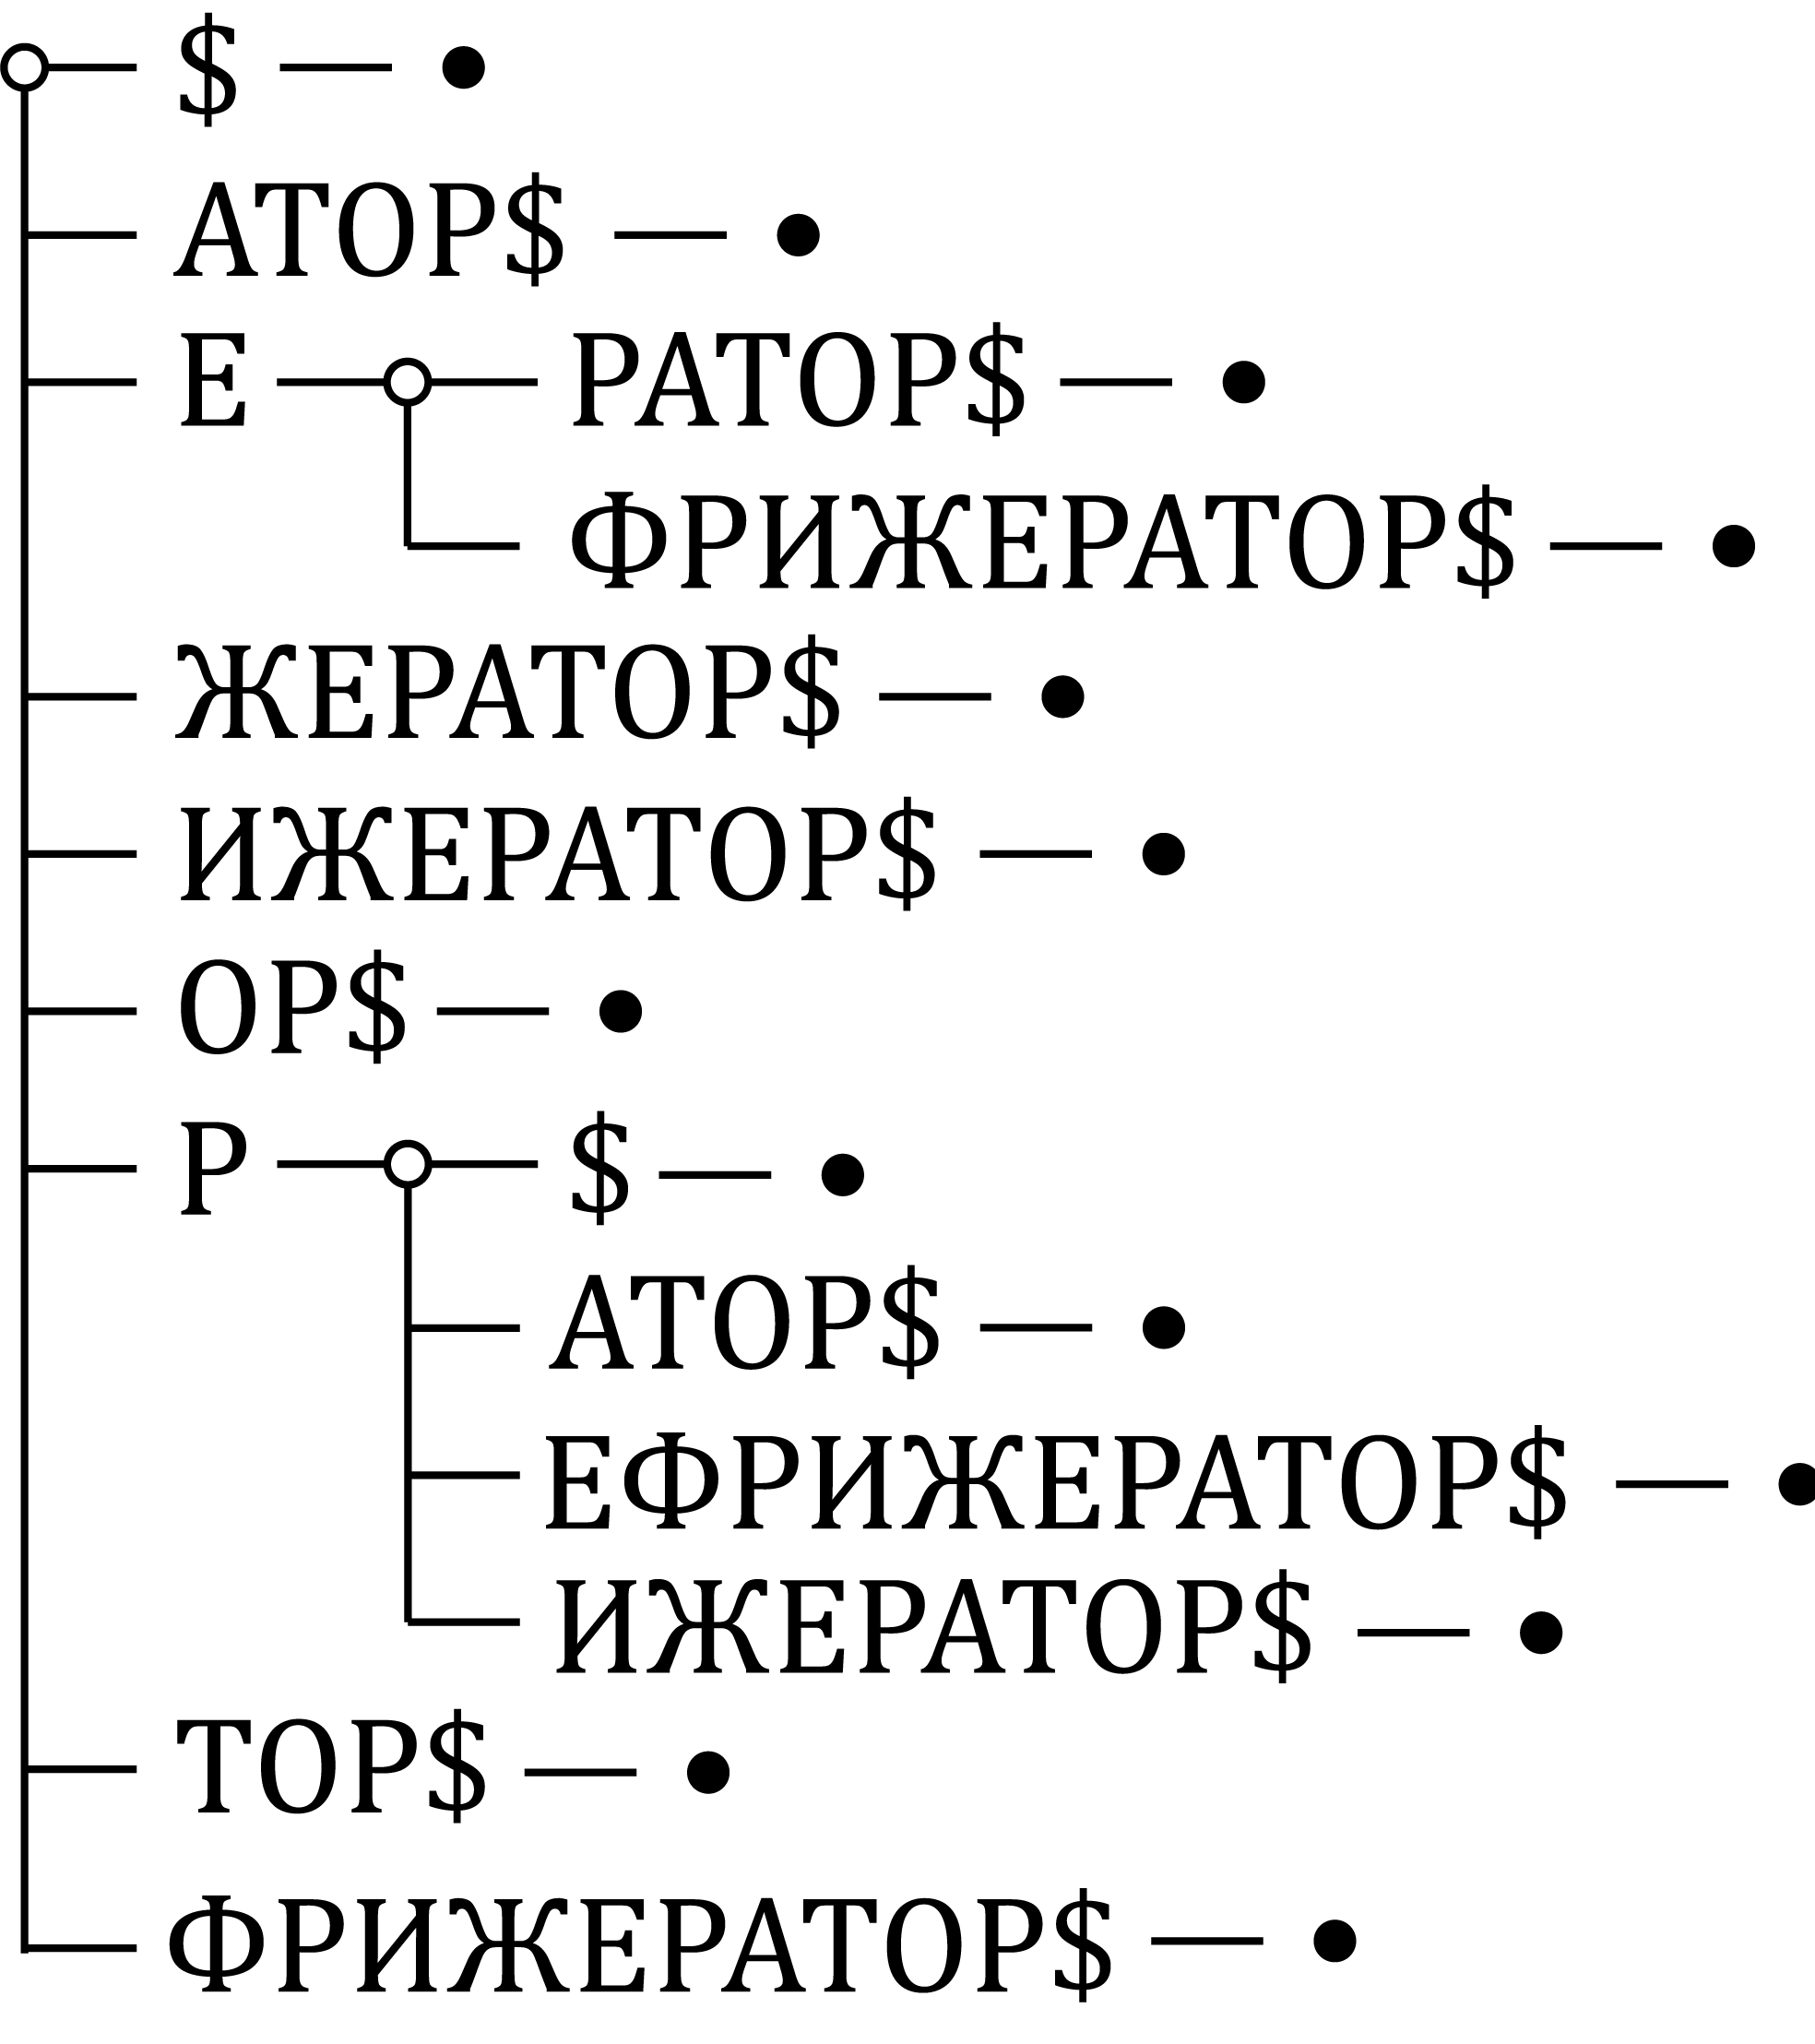
\includegraphics[width=6cm]{pics/23_1.png}
      \centering
  \end{figure}
\end{example}

\begin{remark}
  Размер дерева и память связаны линейно, а также существует алгоритм построения за линию.

  Можно по дереву искать подстроку в строке сравнением посивольно и наибольшую повторяющуюся строку поискам в потомках суффикса (Р)
\end{remark}
\end{document}
